\documentclass[10pt]{beamer}

\usetheme[progressbar=frametitle,numbering=none]{metropolis}
\usepackage{appendixnumberbeamer}

\usepackage{booktabs}

\usepackage{pgfplots}
\usepgfplotslibrary{dateplot}
\usetikzlibrary{calc}
\usepackage[absolute,overlay]{textpos} % for textblock* env

\usepackage{xspace}
\newcommand{\themename}{\textbf{\textsc{metropolis}}\xspace}

\title{multisig, MPC, secret sharing, \ldots}
\subtitle{in-house seminar}
\date{2025-03-XX}
\author{Jeongho Jeon}
\institute{DSRV (All That Node, Custody, Payments, Validator, WELLDONE Studio)}
\titlegraphic{\hfill\includegraphics[height=3.0ex]{dsrv_logo_master_black}}

\begin{document}

\begin{textblock*}{3cm}(0.95\paperwidth,0.97\paperheight)
{\fontsize{2pt}{2.4pt}\selectfont\color{gray}version 20250411}
\end{textblock*}

\maketitle

\begin{frame}[fragile]{Intro}

We sign transactions to prove cryptocurrency ownership or the authority
 to manage it. In many cases, a single private key is used for signing, but
 there is a risk of key loss or leakage. To mitigate this, the key is
 split into multiple parts, and combine them to generate a signature.

\textbf{multisig, MPC wallet, secret sharing, threshold signature}

The terms are frequently misused interchangeably,
 but there are differences.

\end{frame}

\begin{frame}[fragile]{multisig (multi-signature)}

\begin{columns}
\begin{column}{0.7\textwidth}
Typically multisig creates separate signatures using unrelated keys and
concatenates them without any special cryptographic techniques.

\vspace{1em}

Bitcoin has built-in multisig support, \texttt{OP\_CHECKMULTISIG}. Blockchains with smart contracts can implement multisig smart contracts
(e.g., Ethereum's Gnosis Safe). Cosmos SDK supports nested multisigs.

\vspace{1em}

Compared to other methods, it allows for easier weighting.
(e.g., requiring a total of 3 or more votes
when A has 3, B has 2, and both C and D have 1 vote).
\end{column}
\begin{column}{0.3\textwidth}
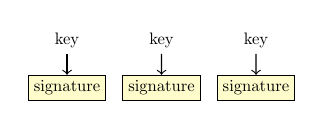
\begin{tikzpicture}[transform shape, scale=0.6]

\node[name=k1] at (0,4) {key} ;
\node[name=k2] at (2,4) {key};
\node[name=k3] at (4,4) {key};

\node[name=s1, draw, fill=yellow, fill opacity=0.2,text opacity=1.0] at (0,3) {signature};
\node[name=s2, draw, fill=yellow, fill opacity=0.2,text opacity=1.0] at (2,3) {signature};
\node[name=s3, draw, fill=yellow, fill opacity=0.2,text opacity=1.0] at (4,3) {signature};

\draw[->] (k1) -- (s1);
\draw[->] (k2) -- (s2);
\draw[->] (k3) -- (s3);
\end{tikzpicture}
\end{column}
\end{columns}

\end{frame}

\begin{frame}[fragile]{MPC (multi-party computation)}

\begin{columns}
\begin{column}{0.7\textwidth}
MPC is a cryptographic field where participants encrypt their secrets,
exchange them, and compute results. For example, encrypted salaries can
be aggregated to calculate the average salary. Beyond signatures, it is
used in voting, auctions, medical data analysis, demographic surveys,
and more.

\vspace{1em}

Each participant signs with their own key, and these signatures are
combined to compute the final signature. It is indistinguishable
whether it was created using a single private key or multiple keys.
Since wallets aggregate multiple signatures, there is only
a single signature on-chain.

\end{column}
\begin{column}{0.3\textwidth}
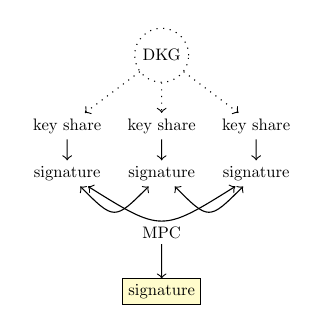
\begin{tikzpicture}[transform shape, scale=0.6]

\node[name=dkg, shape=circle, draw, dotted] at (2,5.5) {DKG};

\node[name=k1] at (0,4) {key share} ;
\node[name=k2] at (2,4) {key share};
\node[name=k3] at (4,4) {key share};

\node[name=s1] at (0,3) {signature};
\node[name=s2] at (2,3) {signature};
\node[name=s3] at (4,3) {signature};
\coordinate (s1') at ($(s1)!0.5!(s2) + (0,-1.0)$);
\coordinate (s2') at ($(s2) + (0,-1.25)$);
\coordinate (s3') at ($(s2)!0.5!(s3) + (0,-1.0)$);

\node at ($(s2') + (0,0)$) {MPC};
%\node[name=mpc, shape=circle, draw] at (2,1.5) {MPC};

\node[name=sf, draw, fill=yellow, fill opacity=0.2,text opacity=1.0] at (2,0.5) {signature};

\draw[->,dotted] (dkg) -- (k1);
\draw[->,dotted] (dkg) -- (k2);
\draw[->,dotted] (dkg) -- (k3);
\draw[->] (k1) -- (s1);
\draw[->] (k2) -- (s2);
\draw[->] (k3) -- (s3);
\draw[<->] (s1) .. controls (s1') .. (s2);
\draw[<->] (s1) .. controls (s2') .. (s3);
\draw[<->] (s2) .. controls (s3') .. (s3);
%\draw[->] (s1') -- (mpc);
\draw[->] ($(s2')+(0,-0.25)$) -- (sf);
%\draw[->] (s3') -- (mpc);
%\draw[->] (mpc) -- (sf);

\end{tikzpicture}
\end{column}
\end{columns}

\end{frame}

\begin{frame}[fragile]{MPC (multi-party computation)}

This enables geographically separated individuals to sign securely online.
 However, participants are often required to be online simultaneously.

\textbf{DKG} (Distributed Key Generation) eliminates the need
to trust a key generator.

Different signature methods (ECDSA, EdDSA, \ldots) require different MPC algorithms.
\end{frame}

\begin{frame}[fragile]{secret sharing}

\begin{columns}
\begin{column}{0.7\textwidth}
It is often referring to the most common Shamir secret sharing method.
A certain number of private key shares are combined to reconstruct
the private key, which is then used to sign.

\vspace{1em}

Similar to MPC, it is indistinguishable whether the signature is made
with one private key or several keys just by a signature.

\vspace{1em}

Since the private keys are combined before signing, it is
signature method agnostic.

\vspace{1em}

There is a risk of key exposure during the signing process.
\end{column}
\begin{column}{0.3\textwidth}
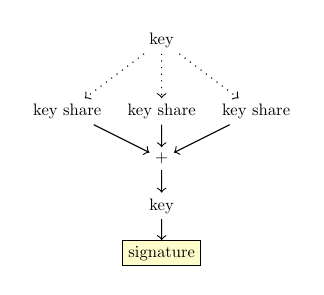
\begin{tikzpicture}[transform shape, scale=0.6]

\node[name=ko] at (2,4.5) {key};

\node[name=k1] at (0,3) {key share} ;
\node[name=k2] at (2,3) {key share};
\node[name=k3] at (4,3) {key share};

\node[name=sss] at (2,2) {$+$};

\node[name=kf] at (2,1) {key};

\node[name=sf, draw, fill=yellow, fill opacity=0.2,text opacity=1.0] at (2,0) {signature};

\draw[->,dotted] (ko) -- (k1);
\draw[->,dotted] (ko) -- (k2);
\draw[->,dotted] (ko) -- (k3);
\draw[->] (k1) -- (sss);
\draw[->] (k2) -- (sss);
\draw[->] (k3) -- (sss);
\draw[->] (sss) -- (kf);
\draw[->] (kf) -- (sf);
\end{tikzpicture}
\end{column}
\end{columns}

\end{frame}

\begin{frame}[fragile]{threshold signature}

Threshold signature is the method where \textit{t} of \textit{n} must
come together to create a signature. Most multisig, MPC, and secret sharing
are threshold signature schemes (TSS).

\end{frame}

\begin{frame}[fragile]{related terms}

\begin{description}
  \item[key rotation] allows for the generation of new key if some keys
   are lost or compromised. Even if there is no issue with keys, we
   change keys periodically for security reasons.
  \item[reconfiguration] regenerates keys when the signing participants
   change.
  \item[signature aggregation] Multiple signatures are aggregated to create
   a single signature. This saves blockchain storage and reduces
   the verification time during blockchain consensus process.
  \item[HSM (Hardware Security Module)] Commonly known
   as a hardware wallet. It signs transactions with stored private key
   without revealing the key itself.
\end{description}

\end{frame}

\begin{frame}[fragile]{related terms}

\begin{description}
  \item[DVT (Distributed Validator Technology)] Validators sign
   blocks they propose and blocks created by others to acknowledge
   the validity of blocks. If validators fails to sign on time
   due to hardware or software issues, they may face penalties
   (inactive slashing). To protect against failures, redundant
   servers may be used, but this introduces the risk of double slashing,
   where two different signature are published. \\
   To address this, multiple servers sign each, and the signatures
   are aggregated to produce a final signature, which is to be published.
   Examples include Obol and SSV on Ethereum. They use BLS signature aggregation within their own signature-making network.
   % https://github.com/ObolNetwork/charon
   % https://github.com/ethereum/ssv
\end{description}

\end{frame}

\end{document}
